\documentclass[10pt,oneside,a4paper]{article}
\usepackage{amsmath,amssymb}
\usepackage{geometry}
\usepackage{multirow}
\usepackage{float}
\geometry{
 a4paper,
 total={170mm,257mm},
 left=7mm,
 right=10mm,
 top=20mm,
 } 
\usepackage{bbm}
\usepackage{amsfonts}
\usepackage{graphicx}
\usepackage{subcaption}
\usepackage{amssymb}
\usepackage{fancyhdr} 
\cfoot{\thepage}
\pagestyle{fancy} 
\fancyhf{}
\fancyhead[LE,RO]{Group 3}
\fancyhead[RE,LO]{\thepage}
\DeclareMathOperator{\E}{\mathbb{E}}



\begin{document}
\begin{flushleft}


\section{Task 1}
\subsection{}
\subsubsection{•}
Finding the first order price sensitivity of Lower Bound of Arithmetic and Geometric Asian options using likelihood ratio method. The LR formulation is given as

\begin{align*}
\mu_{C, \theta} &= \E_\theta \left(C\right) \\
& = \E_\theta\left(f \left(S\right)\right) \\
& = \int_{R^n}^{} f \left(s\right) ds\\
\mu'_{C, \theta}&= \int_{R^n}^{} f \left(s\right)\frac{d \, g_\theta\left(s\right)}{d\theta}ds\\
\end{align*}

by multiplying and dividing $g_\theta\left(s\right)$ the expectation expression is obtained

\begin{align*}
\int_{R^n}^{} f \left(s\right)\frac{d \, g_\theta\left(s\right)}{d \theta} \frac{1}{g_\theta\left(s\right) }g_\theta\left(s\right) ds &= \E_\theta \left(f\left(S\right)\frac{d \, g_\theta\left(S\right)}{d \theta} \frac{1}{g_\theta\left(S\right) }\right)\\
&= \E_\theta \left(f\left(S\right)\frac{d \,ln \, g_\theta \left(S\right)}{d \, \theta}\right)\\
\end{align*}
using the above expression, we take the expected value of the product of the discounted payoff function and the score as the LR first order sensitivity respected to $S_0$. We have the discounted payoff functions for the arithmetic Asian option Lower Bound  and for the geometric Asian option in below.
\begin{align*}
LB_n &= e^{-rT}\left( \frac{1}{n}\sum_{k=1}^{n}S_k - K\right) \mathbbm{1}_{\left( \prod_{k=1}^{n}S_k\right) ^{\frac{1}{n}} >K}\\
G_n &= e^{-rT} max \left(\left(\prod_{k=1}^{n}S_k\right) ^{\frac{1}{n}} - K, 0 \right)\\
\end{align*}

the score for computing an Asian option delta is given as
\begin{align*}
\frac{d \, ln \, g_{S_{0}} (S_1, ...., S_n)}{d S_0} &= \frac{\xi\left(S_1|S_{0}\right)}{S_0 \sigma \sqrt{t_1}}\\
\end{align*}

\begin{align*}
\mu'_{LB, S_0} &= \E _{S_0}\left(e^{-rT}\left( \frac{1}{n}\sum_{k=1}^{n}S_k - K\right)\mathbbm{1}_{\left( \prod_{k=1}^{n}S_k\right) ^{\frac{1}{n} }>K} \cdot \frac{\xi\left(S_1|S_{0}\right)}{S_0 \sigma \sqrt{t_1}} \right)\\
&= \E _{S_0}\left(e^{-rT}\left( \frac{1}{n}\sum_{k=1}^{n}S_k - K\right)\mathbbm{1}_{\left( \prod_{k=1}^{n}S_k\right) ^{\frac{1}{n} }>K} \cdot \frac{ln\frac{S_1}{S_0} - \left(r - \frac{1}{2}\sigma^2\right)\left(t_1 - t_0\right)}{\sigma\sqrt{t_1 - t_0}S_0\sigma\sqrt{t_1}}\right)
\end{align*}

\vspace{5mm}

\begin{align*}
\mu'_{G, S_0} &= \E _{S_0}\left(e^{-rT}\left(\left(\prod_{k=1}^{n}S_k\right) ^{\frac{1}{n}} - K\right)^{+} \cdot \frac{\xi\left(S_i|S_{i-1}\right)}{S_0 \sigma \sqrt{t_1}} \right)\\
\end{align*}
\subsubsection{}
Now, as shown above, the lower bound payoff is discontinuous at $\left( \prod_{k=1}^{n}S_k\right) ^{\frac{1}{n}} =K$. Such that it is not possible to obtain the PW estimator. LR first order sensitivity estimator should be used instead.

\subsection{}
The exact closed formed solutions for the expected Lower Bound and the Geometric payoff are given
\begin{align*}
\E\left(LB_n\right) &= \frac{S_0 e^{-rT}}{n}\sum_{k=1}^{n} e^{\mu_k + \sigma_k^2} \cdot \mathcal{N}\left(b+a_k\right)  - K e^{-rT} \cdot \mathcal{N}\left(b \right)\\
\E\left(G_n\right) &= S_0 e^{\left(r - \frac{\sigma^2}{2} + \frac{\hat{\sigma}^2}{2}\right)\hat{T} - rT} \cdot \mathcal{N}\left(d\right) - K e^{-rT} \cdot \mathcal{N}\left(d - \hat{\sigma}\sqrt{\hat{T}}\right)
\end{align*}
by taking the derivative respected to $S_0$
\begin{align*}
\frac{d \E\left(LB_n\right)}{dS_0} &= \frac{e^{-rT}}{n}\sum_{k=1}^{n} e^{\mu_k + \sigma_k^2} \cdot \mathcal{N}\left(b+a_k\right) + \frac{S_0 e^{-rT}}{n}\sum_{k=1}^{n}e^{\mu_k + \sigma_k^2} \cdot \phi\left(b+a_k\right) \cdot \frac{1}{S_0}\frac{1}{\hat{\sigma}\sqrt{\hat{T}}}\\
& - K e^{-rT} \cdot \phi\left(b \right) \cdot \frac{1}{S_0}\frac{1}{\hat{\sigma}\sqrt{\hat{T}}}\\
 &= \frac{e^{-rT}}{n}\sum_{k=1}^{n} e^{\mu_k + \sigma_k^2} \cdot \mathcal{N}\left(b+a_k\right) + \frac{e^{-rT}}{n}\sum_{k=1}^{n}e^{\mu_k + \sigma_k^2} \cdot \phi\left(b+a_k\right) \cdot \frac{1}{\hat{\sigma}\sqrt{\hat{T}}}\\
& - K e^{-rT} \cdot \phi\left(b \right) \cdot \frac{1}{S_0}\frac{1}{\hat{\sigma}\sqrt{\hat{T}}}\\
\end{align*} 

\vspace{5mm}
\begin{align*}
\frac{d G_n}{dS_0} &= e^{\left(r - \frac{\sigma^2}{2} + \frac{\hat{\sigma}^2}{2}\right)\hat{T} - rT} \cdot \mathcal{N}\left(d\right) + S_0 e^{\left(r - \frac{\sigma^2}{2} + \frac{\hat{\sigma}^2}{2}\right)\hat{T} - rT} \phi \left(d\right) \frac{1}{S_0} \frac{1}{\hat{\sigma}\sqrt{\hat{T}}}\\
& - K e^{-rT} \cdot \phi\left(d - \hat{\sigma}\sqrt{\hat{T}}\right) \cdot \frac{1}{S_0}\frac{1}{\hat{\sigma}\sqrt{\hat{T}}}\\
&= e^{\left(r - \frac{\sigma^2}{2} + \frac{\hat{\sigma}^2}{2}\right)\hat{T} - rT} \cdot \mathcal{N}\left(d\right) +e^{\left(r - \frac{\sigma^2}{2} + \frac{\hat{\sigma}^2}{2}\right)\hat{T} - rT} \phi \left(d\right) \frac{1}{\hat{\sigma}\sqrt{\hat{T}}}\\
& - K e^{-rT} \cdot \phi\left(d - \hat{\sigma}\sqrt{\hat{T}}\right) \cdot \frac{1}{S_0}\frac{1}{\hat{\sigma}\sqrt{\hat{T}}}\\
\end{align*}

where $\mathcal{N}$ is the normal cdf and $\phi$ is the normal pdf.
\subsection{}
\subsubsection{}
The table for the expected lower bounds is the following:

\begin{center}
\begin{table}[ht]
  \large
  \centering
  \begin{tabular}{c|c|*{4}{c|}}
    \multicolumn{5}{c}{K} \tabularnewline
    \cline{2-5}
    \multirow{6}*{\rotatebox{90}{n}} &
&    \bfseries 90 & \bfseries 100 & \bfseries 110  \tabularnewline[1 ex] 
\cline{2-5}
&    \bfseries 4 & 15.032 &  9.2449 &  5.291 \tabularnewline [1ex] 
    \cline{2-5}
&    \bfseries 12 & 14.136 &  8.2345 &  4.3702\tabularnewline [1ex] 
    \cline{2-5}
&    \bfseries 50 & 13.798 &  7.849 &  4.0268 \tabularnewline [1ex] 
    \cline{2-5}
    \cline{2-5}
  \end{tabular}
  \captionof{table}{Expected Lower Bound Values}
\end{table} 
\end{center}

The table for the first sensitivities of the expected lower bounds with respect to S\textsubscript{0} is the following:

\begin{center}
\begin{table}[ht]
  \large
  \centering
  \begin{tabular}{c|c|*{4}{c|}}
    \multicolumn{5}{c}{K} \tabularnewline
    \cline{2-5}
    \multirow{6}*{\rotatebox{90}{n}} &
&    \bfseries 90 & \bfseries 100 & \bfseries 110  \tabularnewline[1 ex] 
\cline{2-5}
&    \bfseries 4 & 0.75587 &   0.57648  &  0.39682 \tabularnewline [1ex] 
    \cline{2-5}
&    \bfseries 12 & 0.76575 &  0.56715 &  0.36875\tabularnewline [1ex] 
    \cline{2-5}
&    \bfseries 50 & 0.77045 &  0.56335 &  0.35684 \tabularnewline [1ex] 
    \cline{2-5}
    \cline{2-5}
  \end{tabular}
    \captionof{table}{Sensitivity of Expected Lower Bound Values}
\end{table} 
\end{center}


\subsubsection{}

The table for the geometric Asian call option prices is the following:

\begin{center}
\begin{table}[ht]
  \large
  \centering
  \begin{tabular}{c|c|*{4}{c|}}
    \multicolumn{5}{c}{K} \tabularnewline
    \cline{2-5}
    \multirow{6}*{\rotatebox{90}{n}} &
&    \bfseries 90 & \bfseries 100 & \bfseries 110  \tabularnewline[1 ex] 
\cline{2-5}
&    \bfseries 4 & 14.525 &  8.8315 &  4.971 \tabularnewline [1ex] 
    \cline{2-5}
&    \bfseries 12 & 13.602 &  7.8021 &  4.0382\tabularnewline [1ex] 
    \cline{2-5}
&    \bfseries 50 & 13.263 &  7.4155 &  3.6945 \tabularnewline [1ex] 
    \cline{2-5}
    \cline{2-5}
  \end{tabular}
\end{table} 
  \captionof{table}{Geometric Asian Call Option Values}
\end{center}

The table for the first sensitivities with respect to S\textsubscript{0} for the geometric Asian option prices is the following:

\begin{center}
\begin{table}[ht]
  \large
  \centering
  \begin{tabular}{c|c|*{4}{c|}}
    \multicolumn{5}{c}{K} \tabularnewline
    \cline{2-5}
    \multirow{6}*{\rotatebox{90}{n}} &
&    \bfseries 90 & \bfseries 100 & \bfseries 110  \tabularnewline[1 ex] 
\cline{2-5}
&    \bfseries 4 & 0.74248 &  0.56288 &  0.38356 \tabularnewline [1ex] 
    \cline{2-5}
&    \bfseries 12 & 0.75131 &  0.55277 &  0.35439\tabularnewline [1ex] 
    \cline{2-5}
&    \bfseries 50 & 0.7558 &  0.54899 &  0.34226 \tabularnewline [1ex] 
    \cline{2-5}
    \cline{2-5}
  \end{tabular}
\end{table} 
  \captionof{table}{Sensitivity of Geometric Asian Call Option Values}
\end{center}

\subsection{}
\subsubsection{}
The table for the Asian call option prices approximated using Monte Carlo simulations using the expected lower bound as a control variate. The table also displays the standard errors and the confidence intervals:
\begin{center}
\begin{tabular}{|c|c|c|c|c|c|c|c|c|c|}
\multicolumn{10}{c}{K} \tabularnewline
\hline
\multirow{3}{*}{} & \multicolumn{3}{c|}{\bfseries 90}  & \multicolumn{3}{c|}{\bfseries 100} & \multicolumn{3}{c|}{\bfseries 110} \\
\cline{2-10}
 & Price & S.E. & C.I. & Price & S.E.. & C.I. & Price & S.E. & C.I \\
\hline
 \bfseries 4 & 15.0371 &  0.00020261 & 15.0367-15.0375 & 9.2492 & 0.00020476 & 9.2488-9.2496 & 5.2960 & 0.00020476 & 5.2956-5.2965   \\
\hline
 \bfseries 12 & 14.1400 & 0.00017697 & 14.1396-14.1403 & 8.2382 & 0.00017074  & 8.2379-8.2385 & 4.3749 & 0.00022525 &4.3745-4.3754 \\
\hline
 \bfseries 50 & 13.8019 & 0.00017443 & 13.8016-13.8023 & 7.8525 & 0.00014983 & 7.8522-7.8528 & 4.0315 & 0.0002129& 4.0311-4.0319 \\
  \hline
\end{tabular}
  \captionof{table}{Approximation with Expected Lower Bound as Control Variate}
\end{center}
 


The table for the Asian call option prices approximated using Monte Carlo simulations using the geometric asian call option with discounted payoff as a control variate. The table also displays the standard errors and the confidence intervals:
\begin{center}
\begin{tabular}{|c|c|c|c|c|c|c|c|c|c|}
\multicolumn{10}{c}{K} \tabularnewline
\hline
\multirow{3}{*}{} & \multicolumn{3}{c|}{\bfseries 90}  & \multicolumn{3}{c|}{\bfseries 100} & \multicolumn{3}{c|}{\bfseries 110} \\
\cline{2-10}
 & Price & S.E. & C.I. & Price & S.E.. & C.I. & Price & S.E. & C.I \\
\hline
 \bfseries 4 & 15.0388 &  0.0020434 & 15.0348-15.0428 & 9.2480 & 0.0018979 & 9.2443-9.2517 & 5.2960 & 0.0018398 & 5.2924-5.2996   \\
\hline
 \bfseries 12 & 14.1386 & 0.0017756 & 14.1352-14.1421 & 8.2395 & 0.0016818  & 8.2362-8.2428 & 4.3736 & 0.0018398 &4.3706-4.3766 \\
\hline
 \bfseries 50 & 13.8030 & 0.0017397 & 13.7996-13.8064 & 7.8525 & 0.0015716 & 7.8494-7.8556 & 4.0326 & 0.0014452 & 4.0298-4.0354 \\ 
  \hline
\end{tabular}
  \captionof{table}{Approximation with Geometric Asian Call Option as Control Variate}
\end{center}

The table with the epsilon values for each strike price and n is the following. It measures which of the two control variates is more efficient:

\begin{center}
\begin{table}[ht]
  \large
  \centering
  \begin{tabular}{c|c|*{4}{c|}}
    \multicolumn{5}{c}{K} \tabularnewline
    \cline{2-5}
    \multirow{6}*{\rotatebox{90}{n}} &
&    \bfseries 90 & \bfseries 100 & \bfseries 110  \tabularnewline[1 ex] 
\cline{2-5}
&    \bfseries 4 & 0.0147 &  0.0162 &  0.0218 \tabularnewline [1ex] 
    \cline{2-5}
&    \bfseries 12 & 0.0120 &  0.0146 &  0.0146\tabularnewline [1ex] 
    \cline{2-5}
&    \bfseries 50 & 0.0126 &  0.0124 &  0.0236 \tabularnewline [1ex] 
    \cline{2-5}
    \cline{2-5}
  \end{tabular}
\end{table} 
  \captionof{table}{Efficiency Values}
\end{center}

It is clear from Table 7 that the using the expected lower bound is more efficient than using the geometric asian call option.

\subsubsection{}
The table for the Asian call option sensitivity with respect to S\textsubscript{0} approximated using Monte Carlo simulations using the sensitivity of the lower bound as a control variate. The table also displays the standard errors and the confidence intervals:
\begin{center}
\begin{tabular}{|c|c|c|c|c|c|c|c|c|c|}
\multicolumn{10}{c}{K} \tabularnewline
\hline
\multirow{3}{*}{} & \multicolumn{3}{c|}{\bfseries 90}  & \multicolumn{3}{c|}{\bfseries 100} & \multicolumn{3}{c|}{\bfseries 110} \\
\cline{2-10}
 & Price & S.E. & C.I. & Price & S.E.. & C.I. & Price & S.E. & C.I \\
\hline
 \bfseries 4 & 0.7639 &  0.00027227 & 0.7633-0.7644 & 0.5856 & 0.00029519 & 0.5850-0.5861 & 0.4071 & 0.00032565 & 0.4064-0.4077   \\
\hline
 \bfseries 12 & 0.7750 & 0.00027437 & 0.7744-0.7755 & 0.5768 & 0.00030602  & 0.5762-0.5774 & 0.3799 & 0.00033711 &0.3793-0.3806 \\
\hline
 \bfseries 50 & 0.7793 & 0.00028271 & 0.7788-0.7798 & 0.5730 & 0.00030121 & 0.5724-0.5736 & 0.3673 & 0.00033988 & 0.3667-0.3680 \\
  \hline
\end{tabular}
  \captionof{table}{Approximation with Expected Lower Bound as Control Variate}
\end{center}
 


The table for the Asian call option sensitivity with respect to S\textsubscript{0} approximated using Monte Carlo simulations using the sensitivity of the geometric Asian option as a control variate. The table also displays the standard errors and the confidence intervals:
\begin{tabular}{|c|c|c|c|c|c|c|c|c|c|}
\multicolumn{10}{c}{K} \tabularnewline
\hline
\multirow{3}{*}{} & \multicolumn{3}{c|}{\bfseries 90}  & \multicolumn{3}{c|}{\bfseries 100} & \multicolumn{3}{c|}{\bfseries 110} \\
\cline{2-10}
 & Price & S.E. & C.I. & Price & S.E.. & C.I. & Price & S.E. & C.I \\
\hline
 \bfseries 4 & 0.7560 &  0.00026752 & 0.7554-0.7565 & 0.5761 & 0.00029418 & 0.5755-0.5767 & 0.3966 & 0.00032115 & 0.3959-0.3972   \\
\hline
 \bfseries 12 & 0.7662 & 0.00028428 & 0.7656 -0.7667 & 0.5671 & 0.00030736  & 0.5664-0.5677 & 0.3686 & 0.00033728 &0.3679-0.3692 \\
\hline
 \bfseries 50 & 0.7710 & 0.00028924 & 0.7704-0.7716 & 0.5630 & 0.00030418 & 0.5624-0.5636 & 0.3577 & 0.0003561 & 0.3570-0.3584 \\ 
  \hline
\end{tabular}
  \captionof{table}{Approximation with Geometric Asian Call Option as Control Variate}


The table with the epsilon values for each strike price and n is the following. It measures which of the two control variates is more efficient:
\newpage
\begin{table}[ht]
  \large
  \centering
  \begin{tabular}{c|c|*{4}{c|}}
    \multicolumn{5}{c}{K} \tabularnewline
    \cline{2-5}
    \multirow{6}*{\rotatebox{90}{n}} &
&    \bfseries 90 & \bfseries 100 & \bfseries 110  \tabularnewline[1 ex] 
\cline{2-5}
&    \bfseries 4 & 0.9858 &  0.97608 &  0.97934 \tabularnewline [1ex] 
    \cline{2-5}
&    \bfseries 12 & 0.87348 &  0.92373 &  0.95308\tabularnewline [1ex] 
    \cline{2-5}
&    \bfseries 50 & 0.90616 &  0.93272 &  0.71096 \tabularnewline [1ex] 
    \cline{2-5}
    \cline{2-5}
  \end{tabular}
    \captionof{table}{Efficiency Values}
\end{table} 

It is clear from Table 10 that the using the sensitivity of the expected lower bound is more efficient than using the geometric asian call option.

\subsubsection{}


\subsection{}
Running the expected lower bound with increasing values of n gives a good approximation for the precise value of the expected value. As expected the higher the value of n the bigger the convergence to the precise value. 

Concretely, the precise value for the expected lower bound is \textbf{7.726961356596341}. Plotting the approximations the following figure can be presented.

\begin{figure}[H]
\centering
        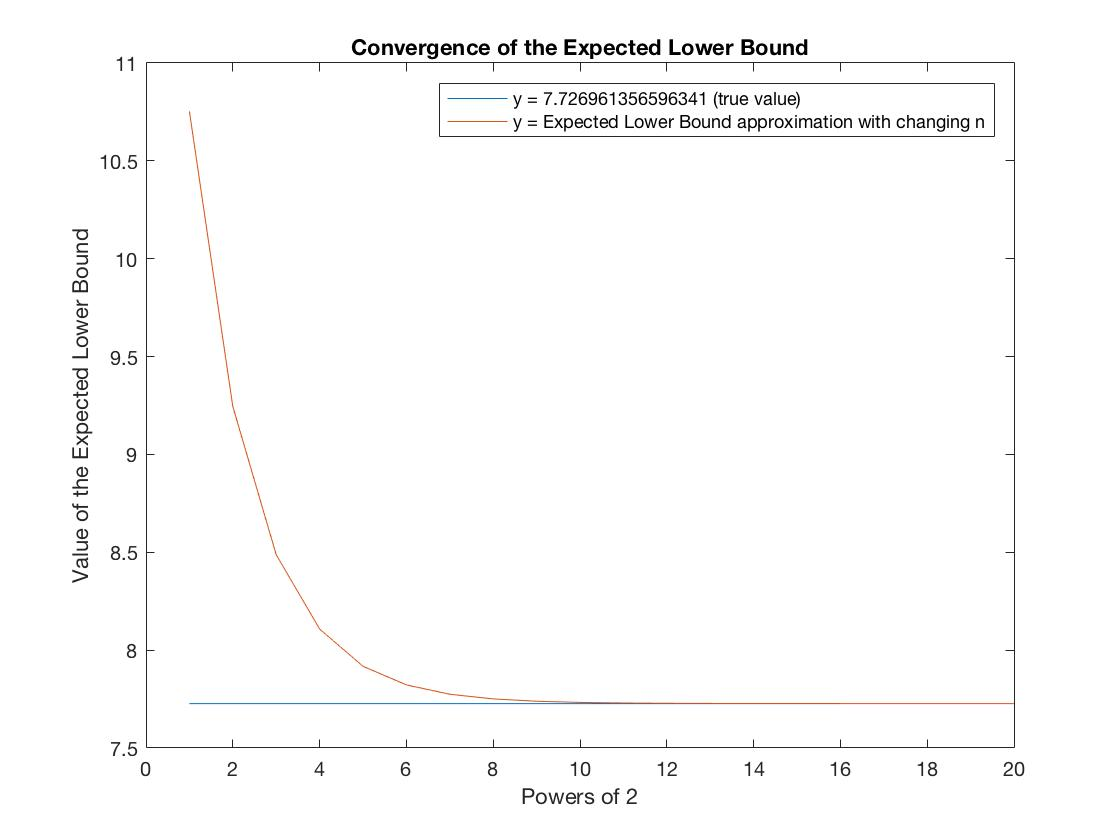
\includegraphics[totalheight=8cm]{convergence.jpg}
        \caption{Convergence of the approximation}
\end{figure}

As it is visible from Figure 1, the approximation gets better when the n is close to the power of 10, and the precision improves as it gets closer to higher n's.
\newline
\newline
The table can be reviewed for further analysis of the precision of the approximation method.

\begin{table}[]
\centering
\begin{tabular}{|c|c|}
\hline
\textbf{i (Power of 2)} & \textbf{Value}     \\ \hline
1                       & 10.752849553377715 \\ \hline
2                       & 9.244949514019062  \\ \hline
3                       & 8.487670434364354  \\ \hline
4                       & 8.107824667550155  \\ \hline
5                       & 7.917532175125288  \\ \hline
6                       & 7.822283197949488  \\ \hline
7                       & 7.774631600352421  \\ \hline
8                       & 7.750798836772930  \\ \hline
9                       & 7.738880689741741  \\ \hline
10                      & 7.732921171871205  \\ \hline
11                      & 7.729941301464144  \\ \hline
12                      & 7.728451338344790  \\ \hline
13                      & 7.727706349800059  \\ \hline
14                      & 7.727333853780493  \\ \hline
15                      & 7.727147605333769  \\ \hline
16                      & 7.727054481001673  \\ \hline
17                      & 7.727007918808091  \\ \hline
18                      & 7.726984637705648  \\ \hline
19                      & 7.726972997149829  \\ \hline
20                      & 7.726967176874716  \\ \hline
\end{tabular}
\captionof{table}{Approximations of the lower bound}
\end{table}
\end{flushleft}
\end{document}
